\newpage 
\section{A Quadratic Trajectory Function (Day 2)}

\myCenteredBox[width=5in,colback=white,sharp corners,]{
    Today you will 
    \begin{itemize}[nosep,label=\checkmark]
        \item Launch \mymm{}s from your catapult.
        \item Time and measure the \mymm~trajectories.
        \item Find a quadratic model that describes the trajectories.
    \end{itemize}
}





\subsection{The General Idea}

The trajectories you tested yesterday are {\bfseries\itshape parabolic}---%
they can be modeled as a quadratic function:
\begin{equation}\label{parabolic-model}
    y = \bm{a}(x-\bm{h})^2 + \bm{k}
\end{equation} 
where 
\begin{itemize}[nosep]
    \item $y$ is the vertical height of the \mymm~trajectory, 
    \item $x$ is the horizontal distance of the \mymm{}s from the catapult, and
\end{itemize}

Today 
{\bfseries\itshape you will find} the values of $\bm{a}$, $\bm{h}$, $\bm{k}$.
Once you find the them, 
you may substitute them into Equation (\ref{parabolic-model}) to get a 
quadratic model of your \mymm~trajectories.





\subsection{DAY 2 Geometry}

There are three points on the parabolic trajectory that are important.
\begin{itemize}[nosep]
    \item $\bm{A}$, the launch point (the $x$-intercept where the catapult is),
    \item $\bm{V}$, the highest point (vertex) of the trajectory, and
    \item $\bm{B}$, the landing point (the $x$-intercept where the \mymm{}s land). 
\end{itemize}

\begin{center}
    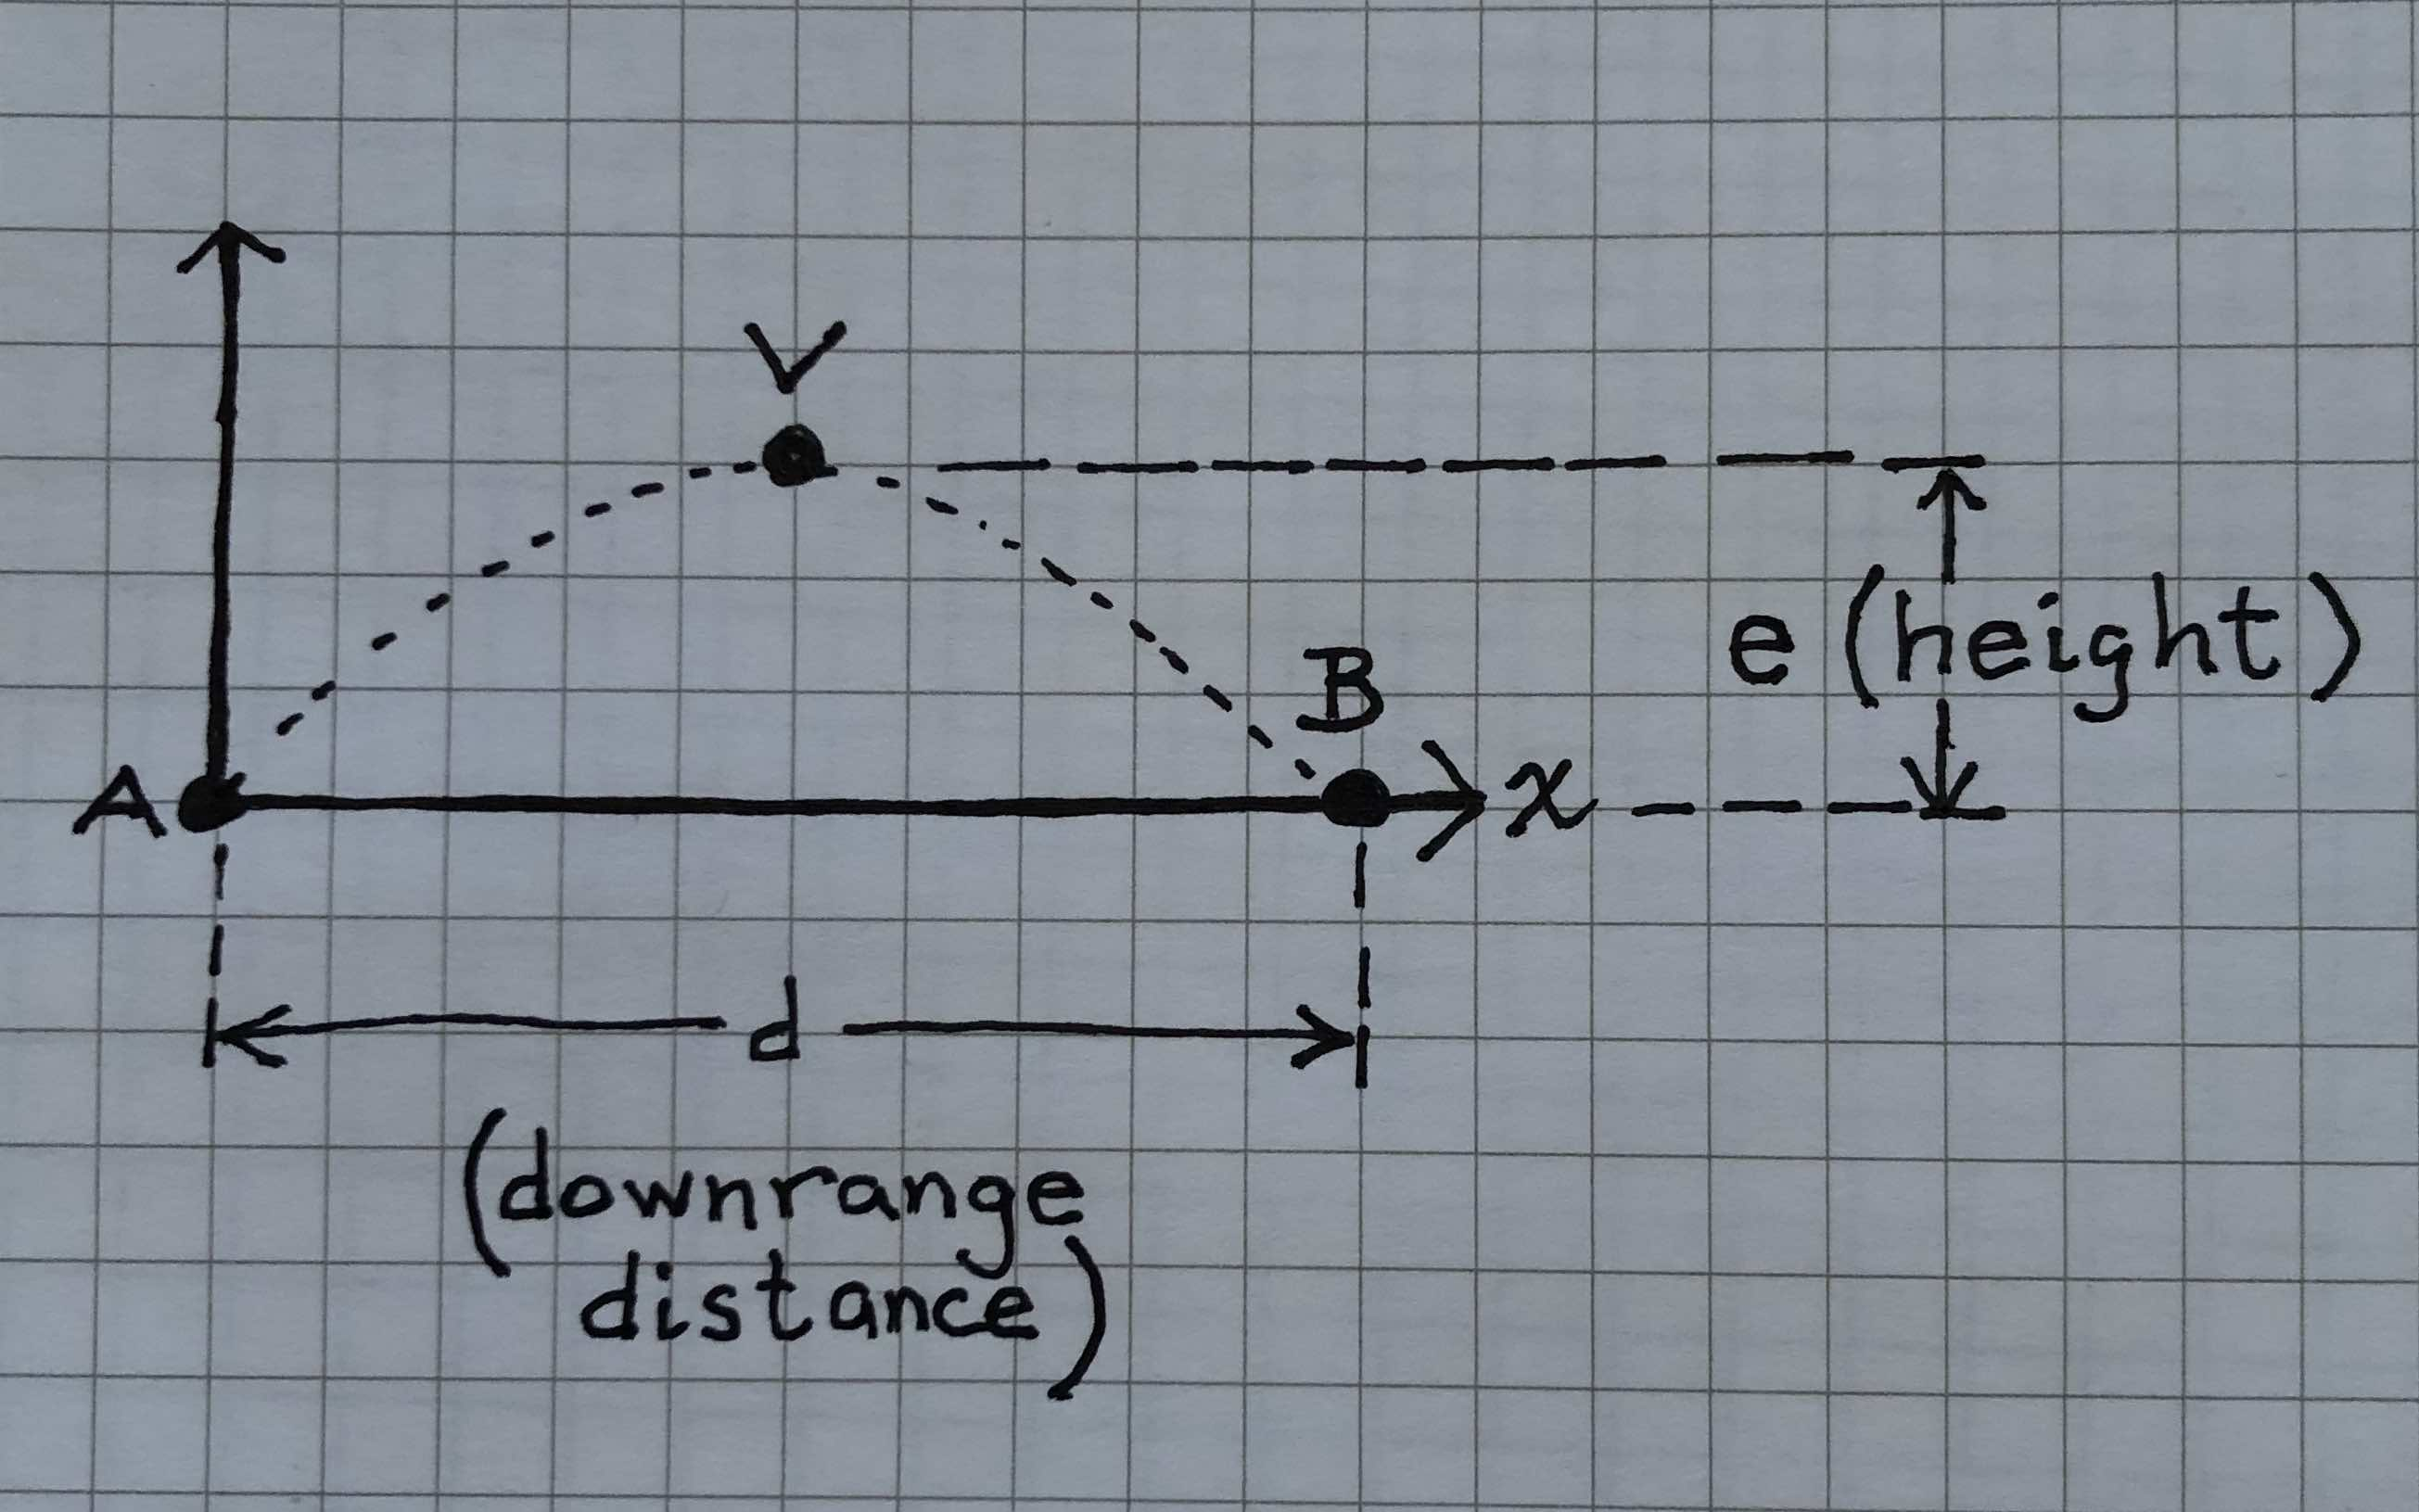
\includegraphics[width=3in]{../AVB.jpg}
\end{center}

You can find the $(x, y)$ coordinates of each of these points, 
once you calculate $d$ and $e$.





\subsection{Launch Data Collection}

Launch your catapult three times.
For each launch,
\begin{itemize}[nosep]
    \item Your group's {\bfseries\itshape timer} person should 
        measure the {\itshape flight time} in seconds using a phone timer.
    \item Your group's {\bfseries\itshape measuring} person should 
        measure {\itshape downrange distance} 
        in centimeters using a yardstick.
    \item Your group's {\bfseries\itshape recording} person should 
        write down the flight time and downrange distance.
\end{itemize}
\myCenteredBox[colback=\myFillinColor]{
    \centering
    \renewcommand{\arraystretch}{1.5}
    \begin{tabular}{c|p{2in}|p{2in}}
        \toprule
        {\itshape launch \#} & {\itshape flight time (sec)} & {\itshape downrange distance (cm)} \\
        \toprule
        1 & & \\
        \midrule
        2 & & \\
        \midrule
        3 & & \\
        \bottomrule
    \end{tabular}
}

Average your measurements.

\begin{tcolorbox}[colback=\myFillinColor,ams align]
    \text{\itshape average downrange distance} = 
    ( 
        \text{\gap{???}} +  \text{\gap{???}} + \text{\gap{???}}
    ) / 3 
    = \text{\gap{???}}
\end{tcolorbox}
\begin{tcolorbox}[colback=\myFillinColor,ams align]
    \text{\itshape average flight time} 
    = 
    ( \text{\gap{???}} +  \text{\gap{???}} + \text{\gap{???}}) / 3 
    = \text{\gap{???}}
\end{tcolorbox}
    


\subsection{Finding $d$ and $e$}

$d$ is the average downrange distance.
\begin{tcolorbox}[colback=\myFillinColor,ams align]
    d 
    = \text{\itshape average downrange distance} 
    = \text{\gap{???}}
\end{tcolorbox}

The time to reach the highest point is one-half the average flight time,
since it occurs in the middle.
\begin{tcolorbox}[colback=\myFillinColor,ams align]
    t_{peak} 
    = \frac{1}{2} (\text{\itshape average flight time})
    = \text{\gap{???}}
\end{tcolorbox}

$e$ comes from phyics: $e = \frac{1}{2}gt^2$, 
where 
$g = 980~cm/s^2$.
\begin{tcolorbox}[colback=\myFillinColor,ams align]
    e & = \frac{1}{2} \cdot g \cdot t^2_{peak} \\
      & = \frac{1}{2} \cdot 980 \cdot (\text{\gap{?????}})^2\\
      & = \text{\gap{?????}}
\end{tcolorbox}





\subsection{The Coordinates of $\bm{A}$, $\bm{V}$, and $\bm{B}$}

The launch point is at the origin.
You know its coordinates.
So $\bm{A}$'s coordinates are
\begin{tcolorbox}[colback=\myFillinColor,ams align]\label{A-coords}
    (x, y)^{}_{\bm{A}} = ( \text{\gap{0}}, \text{\gap{0}})
\end{tcolorbox}
    
The landing point $\bm{B}$ is an $x$-intercept located 
a horizontal distance $d$ from the origin.
But you just found $d$.
So $\bm{B}$'s coordinates are
\begin{tcolorbox}[colback=\myFillinColor,ams align]
    (x, y)^{}_{\bm{B}} = ( \text{\gap{d}}, \text{\gap{0}})
\end{tcolorbox}

The point $\bm{V}$ is located
\begin{itemize}[nosep]
    \item horizontally halfway from $\bm{A}$ to $\bm{B}$,
        which is $\frac{1}{2}d$, and
    \item vertically $e$ units above the $x$-axis.
\end{itemize}
You found $d$ and $e$ above, so $\bm{V}$'s coordinates are 
\begin{tcolorbox}[colback=\myFillinColor,ams align]
    (x, y)^{}_{\bm{V}} &= ( d/2, e)\\ \label{vertex-coords}
    (x, y)^{}_{\bm{V}} &= ( \text{\gap{d/2}}, \text{\gap{e}})
\end{tcolorbox}





\subsection{The Quadratic Trajectory Model}

The quadratic function that models your trajectory 
was mentioned in Equation \ref{parabolic-model} on page~\pageref{parabolic-model}.
We need to find the values of $\bm{a}$, $\bm{h}$, and $\bm{k}$.

The point $\bm{V}$ is the {\bfseries\itshape vertex} with coordinates $(h, k)$.
But you already calculated the coordinates of $\bm{V}$!
(See Equation~\ref{vertex-coords}.)
So $h$ is the $x$-coordinate
and $k$ is the $y$-coordinate 
of $\bm{V}$:
%
\begin{tcolorbox}[colback=\myFillinColor,ams align]\label{h-value}
    h &= \text{\gap{???}}\\
    \label{k-value}
    k &= \text{\gap{???}}
\end{tcolorbox}
%
which means that the quadratic trajectory model (so far) is 
%
\begin{tcolorbox}[colback=\myFillinColor,ams align]\label{model-with-hk}
    y = \bm{a}(x-\text{\gap{h}})^2 + \text{\gap{k}}
\end{tcolorbox}
%
To find the value of $\bm{a}$, 
substitute the coordinates of either $\bm{A}$ or $\bm{B}$  
into this equation.
That will give you and equation that you can solve for $a$.

\myCenteredBox[colback=white,width=3in]{
    Hint: The coordinates of $\bm{A}$ are easiest.
    So use them!
}

The values of $x$ and $y$ at the point $\bm{A}$ 
from Equation~\ref{A-coords} 
are 
\begin{tcolorbox}[colback=\myFillinColor,ams align]
    x_{\bm{A}} &= \text{\gap{0}} \label{xa}\\
    y_{\bm{A}} &= \text{\gap{0}} \label{ya}
\end{tcolorbox}
%
Substitute those two values into Equation~\ref{model-with-hk}.
\begin{tcolorbox}[colback=\myFillinColor,ams align]
    y_{\bm{A}}     &= \bm{a}(x_{\bm{A}}-\text{\gap{h}})^2 + \text{\gap{k}} \label{solve-this-for-a}\\
    \text{\gap{0}} &= \bm{a}(\text{\gap{0}}-\text{\gap{h}})^2 + \text{\gap{k}} \\
    \text{\gap{0}} &= \bm{a}(-\text{\gap{h}})^2 + \text{\gap{k}} \\
    \text{\gap{0}} &= \bm{a} \cdot \text{\gap{???}} + \text{\gap{k}} 
\end{tcolorbox}
%
You can easily solve this for $\bm{a}$. 
Show your work here.
\begin{tcolorbox}[colback=\myFillinColor]
    \vspace{1in}
\end{tcolorbox}
And write your solution here.
\begin{tcolorbox}[colback=\myFillinColor,ams align]\label{a-value}
    \bm{a} = \text{\gap{???}}
\end{tcolorbox}

Your quadratic trajectory model is Equation~\ref{parabolic-model}.
\begin{equation*}
y = \bm{a}(x-\bm{h})^2 + \bm{k}
\end{equation*}

Substituting your values of $\bm{a}$ in Equation~\ref{a-value} 
and $\bm{h}$ and $\bm{k}$ in 
Equation~\ref{model-with-hk},
gives you your quadratic model 
for the catapult trajectories:
%
\begin{tcolorbox}[colback=\myFillinColor,ams align]\label{model-with-ahk}
    y = \text{\gap{a}}(x-\text{\gap{h}})^2 + \text{\gap{k}}
\end{tcolorbox}




\whenHONORS{
\subsection{What About Point $\bm{B}$?}

When you solved Equation~(\ref{solve-this-for-a}) for $\bm{a}$ above, 
you substituted the coordinates of the launch point $\bm{A}$.
Redo the calculation using the coordinates of landing point $\bm{B}$ instead. 
Is this solution for $\bm{a}$ the same as the one above?
\myCenteredBox[colback=\myFillinColor]{
    \centering 
    \qquad
    {\scshape Yes}
    \qquad
    {\scshape No}
    \qquad
    (circle one)
}

Explain why you think this does (or does not) make sense.

\myCenteredBox[colback=\myFillinColor]{
    \vspace{1em}
    \underline{\hspace{\textwidth}}\\[0.5\baselineskip]
    \underline{\hspace{\textwidth}}\\[0.5\baselineskip]
    \underline{\hspace{\textwidth}}\\[0.5\baselineskip]
    \underline{\hspace{\textwidth}}\\[0.5\baselineskip]
    \underline{\hspace{\textwidth}}\\[0.5\baselineskip]
    \underline{\hspace{\textwidth}}\\[0.5\baselineskip]
    \underline{\hspace{\textwidth}}\\[0.5\baselineskip]
    \underline{\hspace{\textwidth}}\\
}
}